%%%%%%%%%%%%%%%%%%%%%%%%%%%%%%%%%%%%%%%%%%%%%%%%%%%%%%%%
%%%%%%%%%%%%%%%%%%%%%%%%%%%%%%%%%%%%%%%%%%%%%%%%%%%%%%%%
\section{Unsupervised Learning}
\label{additional:unsupervised}

%%%%%%%%%%%%%%%%%%%%%%%%%%%%%%%%%%%%%%%%%%%%%%%%%%%%%%%%
\subsection{Bayesian Optimization}
\label{additional:unsupervised:BO}

Frequently we are fortunate enough to have a fairly explicit form of
the objective function $S\left(\bm{\beta}\right)$ to be optimized in order to solve a problem.
However, when $S\left(\bm{\beta}\right)$ is not well-known,
is expensive to compute\footnote{The performance of a machine learning model as a function of its hyperparameters is a classic example of this.
In that case, evaluating $S$ amounts to training the model with a particular set of hyperparameters $\bm{\beta}$,
then determining it's performance on a metric such as ROC AUC.}, or is non-differentiable,
the usual gradient based approaches, such as SGD and Newton's method, break down.
In these cases ``black box''\footnote{Black box as in
we do not have a closed-form expression for $S$, or know $\grad S$.} methods\footnote{Other examples of black box optimizers include
Tree-Structured Parzen Estimators (TPE),
genetic algorithms,
and some additional tree based methods described in \cite{Hutter2011,Hutter2014}.
A TPE is a close relative of Bayesian optimization, making use of the opposite side of Bayes' theorem by
estimating $P\left(\bm{\beta} \mid S\right)$ and $P\left(S\right)$ rather than $P\left(S \mid \bm{\beta}\right)$.
TPEs can accommodate categorical $\beta_{i}$ in a hierarchical manner,
however they can not model interactions between the $\beta_{i}$ \cite{bissuel_2019,NIPS2011_4443}.},
such as Bayesian optimization, may be used instead.

In Bayesian optimization\footnote{Generalized
formally as Sequential Model-Based Optimization (SMBO) \cite{NIPS2011_4443}.} \cite{Brochu2010,1301.1942,Borisyak,NIPS2011_4443},
$S$ is approximated by a well-known surrogate function\footnote{Also known as a response surface.}.
The surrogate typically is a Gaussian process (GP),
but can be any well-behaved regressor such as
a Random Forest or Boosted Decision Tree (BDT).
GPs \cref{eq:additional:unsupervised:BO:GP} are
extensions of Gaussian distributions which return a Gaussian at any point along their domain.
They are parameterized by a mean function\footnote{For convenience,
the prior $m\left(\bm{x}\right)$ is usually assumed to be zero, $m\left(\bm{x}\right)=0$.}, $m\left(\bm{x}\right)$,
and covariance function, $k\left(\bm{x}_{i}, \bm{x}_{j}\right)$,
\ie kernel\footnote{The kernel of the GP is a hyperparameter to be chosen in advance.
Standard kernel choices include
the radial basis function kernel $k\left(\bm{x}_{i}, \bm{x}_{j}\right) = \exp\left(-\frac{1}{2\sigma^{2}}\norm{\bm{x}_{i}-\bm{x}{j}}^{2}\right)$,
Mat\'{e}rn kernel,
and white noise kernel $k\left(\bm{x}_{i}, \bm{x}_{j}\right) \propto \delta_{ij}$.},
instead of a constant mean $\mu$ and variance $\sigma^{2}$.
An illustration of a GP is provided in \cref{fig:additional:unsupervised:BO:GP_ex}.

\begin{equation}\label{eq:additional:unsupervised:BO:GP}
f\left(\bm{x}\right) \sim \mathcal{GP}\left(m\left(\bm{x}\right), k\left(\bm{x}_{i}, \bm{x}_{j}\right)\right).
\end{equation}

\begin{figure}[H] % TODo might want to eventually remove
\centering
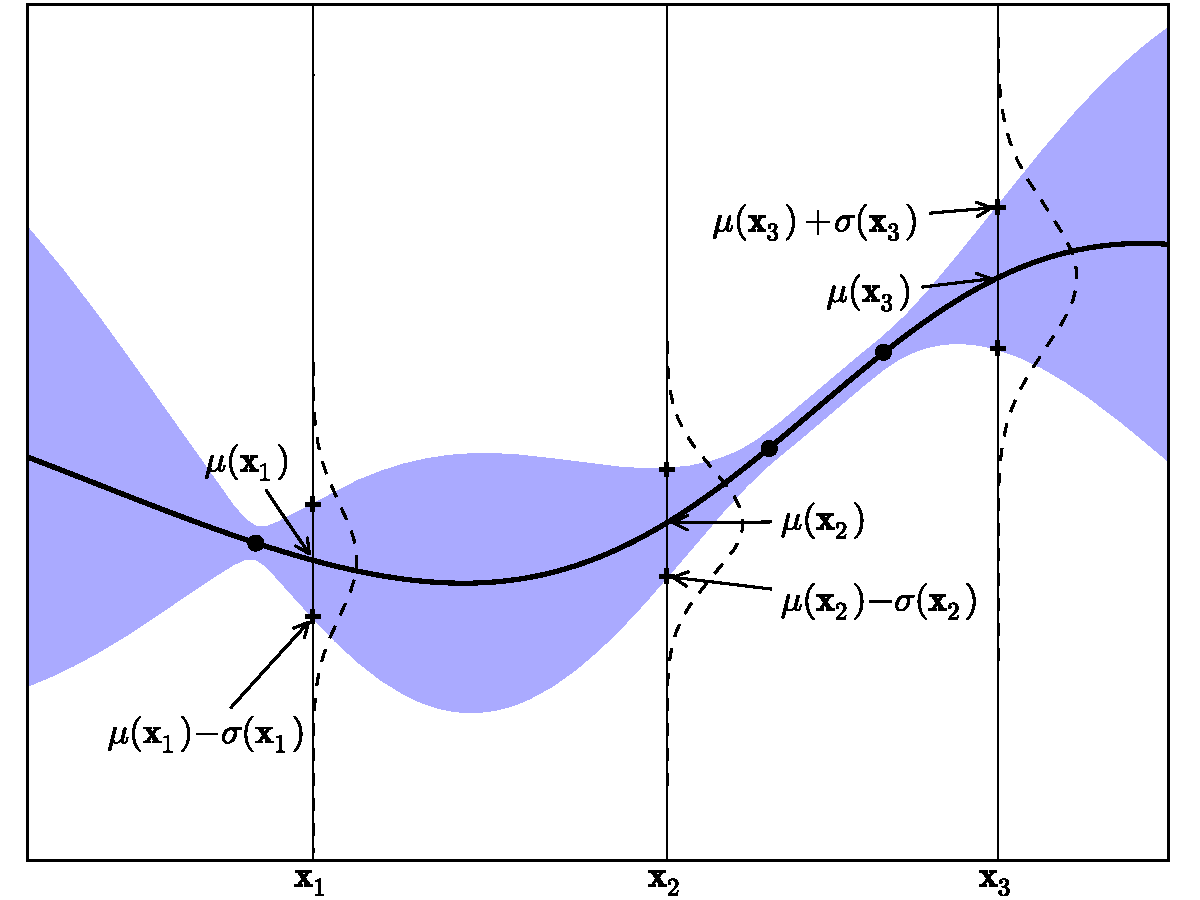
\includegraphics[width=0.85\textwidth]{figures/ml/gp}
\caption{
Illustration of a Gaussian process (GP) in 1D \cite{Brochu2010}.
Note that at any point $\bm{x}_{1}$, $\bm{x}_{2}$, $\bm{x}_{3}$ the GP
returns a Gaussian distribution characterizing the estimated mean and uncertainty on the
unknown true function, \ie the objective function $S\left(\bm{\beta}\right)$ in the case of Bayesian optimization.
}
\label{fig:additional:unsupervised:BO:GP_ex}
\end{figure}

The surrogate function is initially fit to
a random sample of $\bm{\beta}$, $S\left(\bm{\beta}\right)$ points.
From this prior, Bayesian optimization
operates by iteratively sampling $S\left(\bm{\beta}\right)$ and updating
the posterior surrogate function as each new piece of information is gained.
An acquisition function, $u\left(\cdot\right)$, directs the sampling,
estimating where $S\left(\bm{\beta}\right)$ may be large
due to a high predicted value, large uncertainty, or some combination of the two.
The exploration-exploitation tradeoff inherent in $u\left(\cdot\right)$
can be tuned in various ways, see Section 2.3 of \cite{Brochu2010} for a full description\footnote{Common types of acquisition function include the
Expected Improvement (EI);
$\text{EI}\left(\bm{\beta}\right) = \expvalE{\max\left(0,\,S\big(\bm{\beta}\big) - S\big(\hat{\bm{\beta}}\big)\right)}$
where $S\big(\hat{\bm{\beta}}\big)$ is the current optimal value of $S$,
Upper Confidence Bound (UCB);
$\text{UCB}\left(\bm{\beta}\right) = E_{\text{GP}} \left(\bm{\beta}\right) + \kappa\,\text{var}_{\text{GP}} \left(\bm{\beta}\right)$ where the mean and variance are of the GP and $\kappa$ sets the exploration-exploitation tradeoff,
and Maximum Probability of Improvement (MPI).}.
The iterative nature of Bayesian optimization is illustrated in \cref{fig:additional:unsupervised:BO:BO_ex}.
An accessible implementation of Bayesian optimization is available in \skopt \cite{scikit-optimize,Borisyak}.

\begin{figure}[H] % TODo might want to eventually remove
\centering
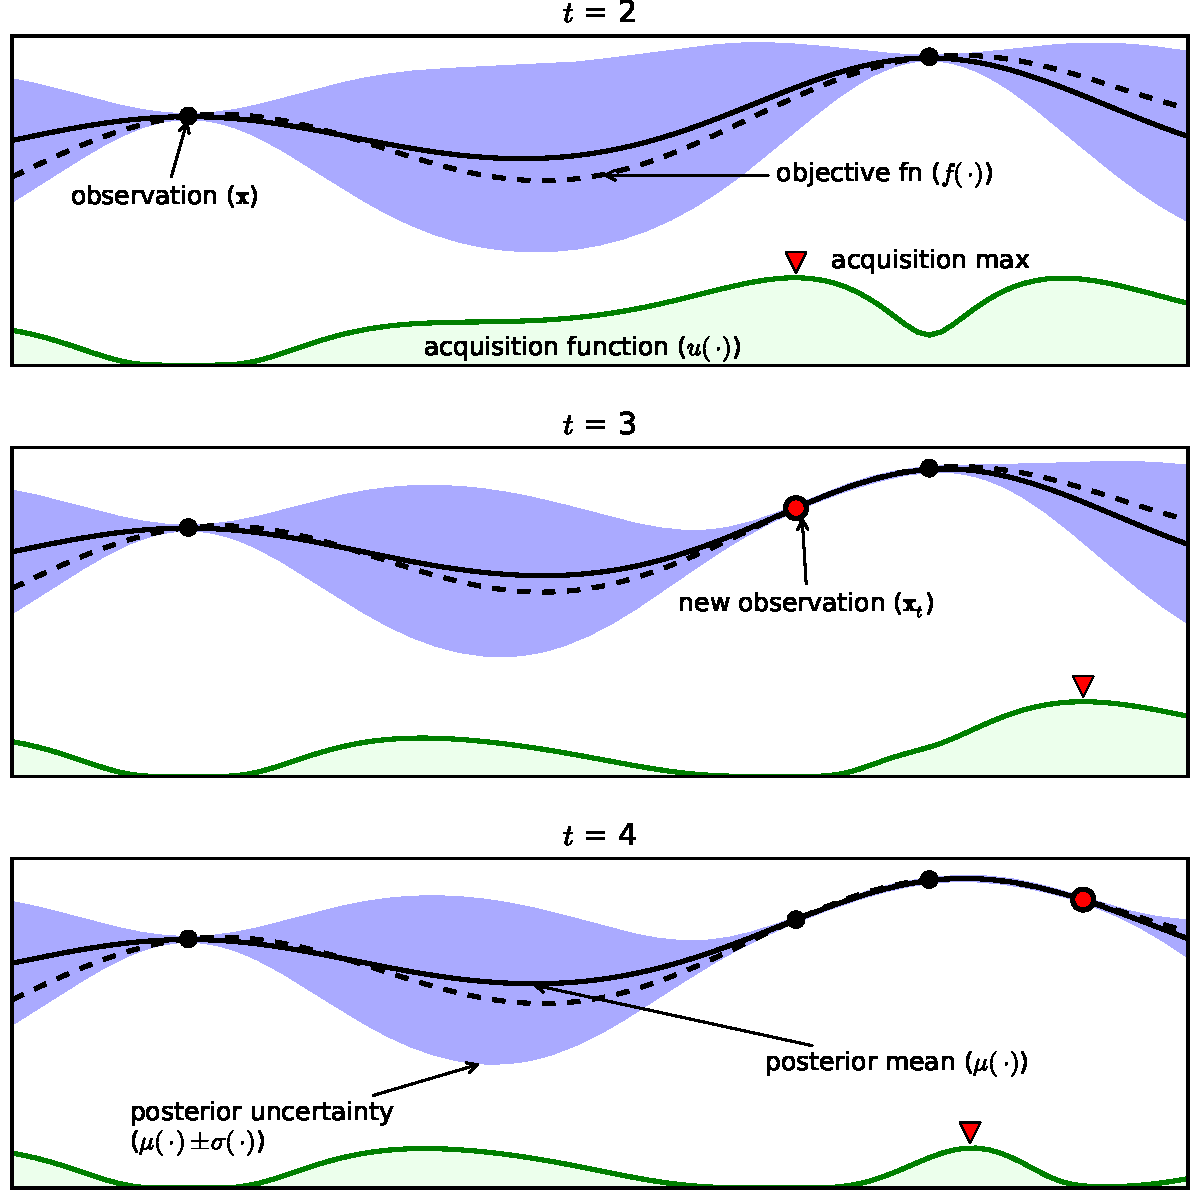
\includegraphics[width=0.85\textwidth]{figures/ml/toyGPtext3}
\caption{
Illustration of Bayesian optimization over three iterations in a toy 1D maximization problem \cite{Brochu2010}.
Note that the maximum of the acquisition function $u\left(\cdot\right)$
locates where $S\left(\bm{\beta}\right)$ should be sampled next.
The GP estimated posterior distribution of $S\left(\bm{\beta}\right)$
and $u\left(\cdot\right)$ are then updated.
This iterative process is repeated until the estimated maximum is satisfactory.
}
\label{fig:additional:unsupervised:BO:BO_ex}
\end{figure}

%%%%%%%%%%%%%%%%%%%%%%%%%%%%%%%%%%%%%%%%%%%%%%%%%%%%%%%%
\subsection{Gaussian Mixture Model (GMM)}
\label{additional:unsupervised:GMM}
% TODO

%%%%%%%%%%%%%%%%%%%%%%%%%%%%%%%%%%%%%%%%%%%%%%%%%%%%%%%%
\subsection{Louvain Method}
\label{additional:unsupervised:louvain}

When working with a graph, \ie network, based dataset
we can use the Louvain\footnote{Named for the location of the author's university in Louvain-la-Neuve, Belgium.} method \cite{louvain}
to detect related clusters, \ie communities,
of nodes by optimizing the graph's modularity.
The modularity $Q$ of a graph $G$ with a given set of clusters $C$
is a measure of the graph's degree of clustering;
being the fraction of edges within the clusters
minus the expected fraction if the edges were randomly distributed.
In short, we can think of $Q$ as a measure of
the density of interior to exterior edges of the clusters.
$Q$ ranges from \num{-0.5} for relatively uncluttered graphs
to \num{1} for fully clustered graphs.
We can compute the modularity $Q$ of $G$ as:

\begin{equation} \label{eq:unsupervised:louvain:modularity}
Q\left(G\right) = \frac{1}{2 W_{G}} \sum_{ij \in G} \bigg(w_{ij} - \gamma \frac{W_{i} W_{j}}{2 W_{G}}\bigg) \delta\left(c_{i},\,c_{j}\right)
\end{equation}

\noindent where\footnote{Note $w_{ij}=1$ for an unweighted graph, and $2 W_{G} = \sum_{ij \in G} w_{ij}$ accounts for double counting edges.}
$w_{ij}$ is the edge weight between nodes $i$ and $j$,
$W_{i}$ is the sum of edge weights of node $i$,
$W_{G}$ is the total edge weight of the graph,
$c_{i} \in C$ is the cluster of node $i$,
and $0 < \gamma$ is a resolution hyperparameter.

The Louvain method constructs $C$ by maximizing $Q$ in an iterative two phase process as shown in \cref{fig:louvain}.
In the first phase, we define each node $n_{i} \in G$ to be its own cluster $c_{i}$.
We then merge each $c_{i}$ with the neighboring $c_{j}$, $0 < w_{ij}$, which maximizes $\Delta Q$.
If $\max\left(\Delta Q\right) = 0$ we leave $c_{i}$ unmerged.
After all clusters have been merged and $Q$ is at a local maximum we enter the second phase.
Here a new graph $G'$ is constructed by making each cluster $c_{i}$ into a node $n'_{i} \in G'$.
The old weights of $G$ are summed to become the new weights $w'_{ij}$,
with intra-cluster weights becoming self-loops $w'_{ii}$ in $G'$.
We return to the first phase and repeat until $Q$ has been maximized.

\begin{figure}
\centering
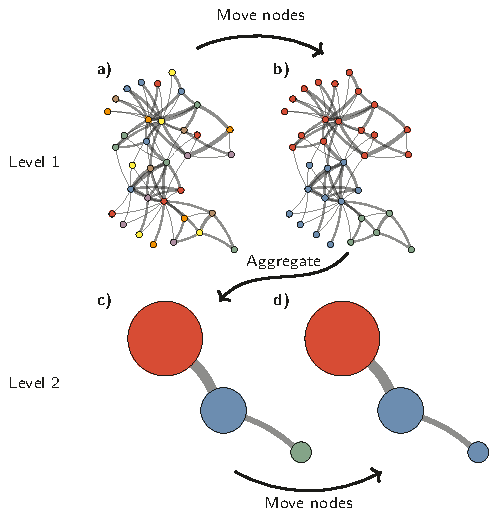
\includegraphics[width=0.5\textwidth]{figures/ml/louvain_algo}
\caption{
Illustration of the two iterative phases of the Louvain method \cite{leiden}.
}
\label{fig:louvain}
\end{figure}

The resolution parameter $\gamma$ controls the number and size of clusters, $\gamma =1$ by default.
The location of $\gamma$ depends on the text and implementation,
but here $1 < \gamma$ ($\gamma < 1$) favors more (fewer) clusters with fewer (more) constituent nodes.
The \texttt{python-louvain}
\href{https://python-louvain.readthedocs.io/en/latest/}{package} \cite{python-louvain}
implements the Louvain method for \texttt{networkx} \cite{networkx}
\href{https://networkx.org/}{based graphs}.
Community detection in large networks is an important problem for social networks and other use cases,
making this an active area of research.
For example, one proposed improvement to the Louvain method is the Leiden algorithm \cite{leiden}.

%%%%%%%%%%%%%%%%%%%%%%%%%%%%%%%%%%%%%%%%%%%%%%%%%%%%%%%%
\subsection{Variational Autoencoders (VAE)}
\label{additional:unsupervised:VAE}
% TODO

%%%%%%%%%%%%%%%%%%%%%%%%%%%%%%%%%%%%%%%%%%%%%%%%%%%%%%%%
\subsection{Support Vector Clustering}
\label{additional:unsupervised:SVC}
% TODO

